\documentclass[10pt,twocolumn]{article}
\usepackage[letterpaper,top=0.75in,bottom=1in,left=0.625in,right=0.625in,columnsep=0.25in]{geometry}
\usepackage{mathptmx}
\usepackage[T1]{fontenc}
\usepackage{amsmath,graphicx,booktabs,cite,titlesec,array}
\graphicspath{{../figures/}}
\usepackage[font=footnotesize,labelfont=normal,labelsep=period]{caption}
\setlength{\parindent}{0.15in}
\renewcommand{\figurename}{Fig.}
\renewcommand{\tablename}{TABLE}\renewcommand{\thetable}{\Roman{table}}
\setlength{\parskip}{0pt}
\pagestyle{empty}
\renewcommand{\thesection}{\Roman{section}}
\renewcommand{\thesubsection}{\Alph{subsection}}
\titleformat{\section}{\centering\normalfont\small\scshape}{\thesection.}{0.5em}{}
\titleformat{\subsection}{\normalfont\itshape}{\thesubsection.}{0.5em}{}
\titlespacing*{\section}{0pt}{10pt}{4pt}
\titlespacing*{\subsection}{0pt}{6pt}{2pt}
\renewcommand{\arraystretch}{1.1}
\newcommand{\Rsun}{R_{\odot}}
\newcommand{\Rearth}{R_{\oplus}}

\begin{document}

\twocolumn[{
\begin{center}
{\LARGE Exoplanet Hunters: Transit Analysis of STAC-1, STAC-2 and STAC-3\\[2pt]}
{\large Operation Dim Star, STAC Wars Problem Set 3\\[8pt]}
{\normalsize Team [your team name]\\
\textit{[Your names, institution, e-mail]}}
\end{center}
\vspace{2pt}
\begin{center}
\begin{minipage}{0.93\textwidth}
\small\noindent\textbf{\textit{Abstract}---}We looked at the relative brightness of three stars to see whether anything is passing in front of them. All three show repeating dips. We estimate periods of about 4.25 d, 80 d and 38 d, transit depths of 0.30\,\%, 0.10\,\% and 0.088\,\%, and planet radii of roughly 6.0, 2.8 and 1.6 Earth radii. Kepler's third law puts the planets at 0.051, 0.337 and 0.176 AU. STAC-1\,b is a hot Neptune-sized planet that is far too close to its star. STAC-2\,b is warm, but its size suggests a thick gas envelope. STAC-3\,b is the smallest and, in our judgement, the best target for follow-up. Being in the habitable zone is not the same as being habitable, and we say below why that matters here.\\[4pt]
\textbf{\textit{Index Terms}---}exoplanets, transit photometry, Kepler's third law, habitable zone, M dwarf
\end{minipage}
\end{center}
\vspace{6pt}
}]

\section{Introduction}
When a planet crosses the disc of its star as seen from Earth, it blocks a small fraction of the light. A space telescope has recorded the relative brightness of three stars, and our job is to decide whether the dips are real planets, how big and how far out those planets are, and which one deserves a closer look. Transit photometry of this kind is the same technique used by the Kepler mission \cite{borucki,winn}. We follow the order of the brief: detection (Section~II), size (Section~III), orbit (Section~IV) and the choice of the best candidate (Section~V).

Stellar properties are taken from the data sheet and listed in Table~I.

\begin{table}[h]
\centering
\caption{Host star properties (given)}
\small
\begin{tabular}{lccc}
\toprule
 & STAC-1 & STAC-2 & STAC-3\\
\midrule
Mass ($M_\odot$) & 1.00 & 0.80 & 0.50\\
Radius ($R_\odot$) & 1.00 & 0.80 & 0.50\\
Luminosity ($L_\odot$) & 1.00 & 0.40 & 0.08\\
$T_\mathrm{eff}$ (K) & 5800 & 5000 & 3800\\
\bottomrule
\end{tabular}
\end{table}

\subsection*{Assumptions}
We assume one planet per star, a circular orbit, an edge-on view so the planet crosses the middle of the disc, no limb darkening, a planet that is dark and small compared with its star, and a planet mass that is negligible next to the stellar mass. The brief writes the depth relation as $\delta\approx(R_s/R_p)^2$. That is upside down, because a planet smaller than its star would give $\delta>1$. The physically correct form is $\delta\approx(R_p/R_s)^2$, and we use it throughout.

\section{Detection of the Exoplanets}

\subsection{Reading the light curves}
Fig.~1 shows the three data sets. Every star sits at a flat baseline of 1.0000 with occasional drops, and the drops in each star are all the same depth. That is the signature we want.

\begin{figure}[t]
\centering
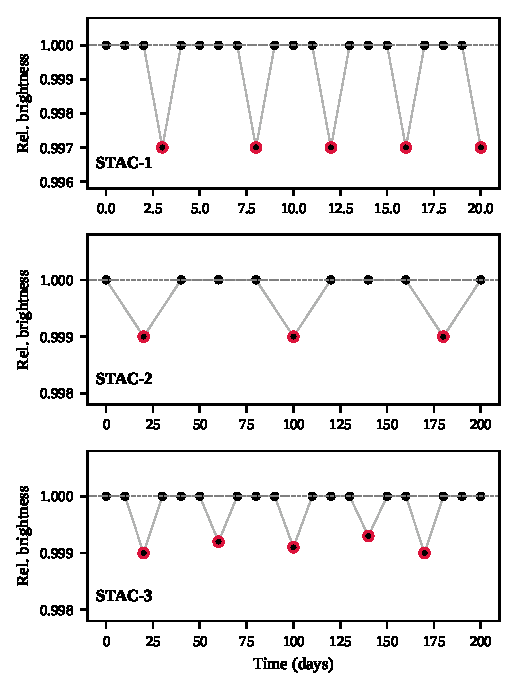
\includegraphics[width=\columnwidth]{lc.pdf}
\caption{Relative brightness of the three stars. Circled points are the in-transit measurements. Note the different time scales.}
\end{figure}

\textbf{STAC-1.} The telescope sampled once per day. Brightness falls to 0.9970 on days 3, 8, 12, 16 and 20, and is 1.0000 on all other days. The gaps between dips are 5, 4, 4 and 4 days. The average spacing is $(20-3)/4=4.25$ d, so we take
\begin{equation}
P_1\approx 4.25\ \text{d}\quad(\text{range }4.0\text{--}4.3\ \text{d}).
\end{equation}
The one 5-day gap is a sampling effect. A transit lasts under a day, so with daily sampling it can fall between two observations. A strict 4.0-day period would not reproduce the gap between days 3 and 8, whereas 4.25 d does (a transit lasting about 0.8 d, starting near days 2.95, 7.2, 11.45, 15.7 and 19.95, is caught by exactly the observations on days 3, 8, 12, 16 and 20 and by no others).

\textbf{STAC-2.} Samples are 20 days apart. Dips to 0.9990 appear at days 20, 100 and 180, so
\begin{equation}
P_2 = 100-20 = 180-100 = 80\ \text{d}.
\end{equation}
Shorter periods that divide 80 d (40 d, for example) would have put a dip at days 60 and 140, and those readings are 1.0000. Because only every 20th day is sampled, we cannot rule out an unusual period that happens to miss all other samples, so 80 d is our best estimate, not a precise measurement.

\textbf{STAC-3.} Samples are 10 days apart. Dips appear at days 20, 60, 100, 140 and 170, with depths 0.9990, 0.9992, 0.9991, 0.9993 and 0.9990. The first four are spaced by exactly 40 d, but the fifth falls only 30 d after the fourth, and day 180 is flat. A strict 40 d period would predict a dip at day 180, so it does not fit. A least-squares line through (transit number, day) gives a slope of 38.0 d, and the plain average spacing $(170-20)/4$ gives 37.5 d. We adopt
\begin{equation}
P_3\approx 38\ \text{d}\quad(\text{range }37.5\text{--}40\ \text{d}).
\end{equation}
The scatter is what you would expect from 10-day sampling of a short transit, and the choice within this range changes the orbit by only a few percent (Section~IV).

\subsection{Transit depth}
Using $\delta=(F_\text{normal}-F_\text{transit})/F_\text{normal}$ with $F_\text{normal}=1.0000$:
\begin{align}
\delta_1 &= 1-0.9970 = 0.0030\ (0.30\,\%),\\
\delta_2 &= 1-0.9990 = 0.0010\ (0.10\,\%),\\
\delta_3 &= \tfrac{1}{5}\bigl[(10+8+9+7+10)\times10^{-4}\bigr] = 0.00088.
\end{align}
For STAC-3 we averaged the five dips because the individual values differ slightly (0.0007 to 0.0010), probably from noise or from sampling a point partway through ingress or egress. For STAC-1 and STAC-2 every dip has the same depth.

\subsection{Why a periodic dip suggests a planet}
A planet is a dark body that blocks part of the stellar disc each time it passes in front. This produces a short, flat-bottomed dip that repeats at the orbital period and always has about the same depth, because the planet's size does not change. Starspots can also dim a star, but they come and go as the star rotates and rarely repeat with a constant depth. Instrument glitches would not follow a regular period. A repeating, equal-depth, regular signal is therefore the planetary explanation. It is not proof, since an eclipsing binary can mimic a transit, but the small depths here (at most 0.3\,\%) are too shallow for a stellar companion eclipsing a normal star. \emph{Conclusion: all three stars host a transiting planet.}

\begin{table}[h]
\centering
\caption{Detection summary}
\small
\begin{tabular}{lccc}
\toprule
 & STAC-1 & STAC-2 & STAC-3\\
\midrule
Planet detected & Yes & Yes & Yes\\
Dips seen & 5 & 3 & 5\\
Period $P$ (d) & 4.25 & 80 & 38\\
Depth $\delta$ & 0.0030 & 0.0010 & 0.00088\\
\bottomrule
\end{tabular}
\end{table}

\section{Planet Size}
Rearranging $\delta=(R_p/R_s)^2$ gives $R_p=R_s\sqrt{\delta}$. With $R_\odot=696{,}000$ km and $R_\oplus=6371$ km:

\textbf{STAC-1\,b.}\ $R_s=696{,}000$ km, $\sqrt{0.0030}=0.05477$,
\begin{equation}
R_p = 696{,}000\times0.05477 \approx 38{,}100\ \text{km}\approx 5.98\,\Rearth.
\end{equation}

\textbf{STAC-2\,b.}\ $R_s=0.8\times696{,}000=556{,}800$ km, $\sqrt{0.0010}=0.03162$,
\begin{equation}
R_p = 556{,}800\times0.03162 \approx 17{,}600\ \text{km}\approx 2.76\,\Rearth.
\end{equation}

\textbf{STAC-3\,b.}\ $R_s=0.5\times696{,}000=348{,}000$ km, $\sqrt{0.00088}=0.02966$,
\begin{equation}
R_p = 348{,}000\times0.02966 \approx 10{,}300\ \text{km}\approx 1.62\,\Rearth.
\end{equation}
Using the extreme depths 0.0007 and 0.0010 for STAC-3 gives 1.45 and 1.73\,$\Rearth$, so the uncertainty is roughly $\pm0.15\,\Rearth$.

\textbf{Classification.} We use these approximate bins: Earth-sized below $1.25\,\Rearth$, Super-Earth 1.25 to 4, Neptune-sized 4 to 10, and Jupiter-sized above 10 (Jupiter is about $11\,\Rearth$). The result is shown in Table~III.

\begin{table}[h]
\centering
\caption{Planet radii and classification}
\small
\begin{tabular}{lccc}
\toprule
Planet & $R_p$ (km) & $R_p/\Rearth$ & Class\\
\midrule
STAC-1\,b & 38,100 & 5.98 & Neptune-sized\\
STAC-2\,b & 17,600 & 2.76 & Super-Earth\\
STAC-3\,b & 10,300 & 1.62 & Super-Earth\\
\bottomrule
\end{tabular}
\end{table}

STAC-2\,b sits near the boundary where researchers often switch from ``super-Earth'' to ``mini-Neptune'', so the label should be read loosely.

\section{Planetary Orbits}
Rearranging $P^2=a^3/M$ gives $a=(M P^2)^{1/3}$, with $P$ converted to years by dividing by 365.25. One AU is $149.6\times10^6$ km.

\textbf{STAC-1\,b.}\ $P=4.25/365.25=0.011636$ yr, $P^2=1.354\times10^{-4}$, $M=1.00$:
\begin{equation}
a=(1.00\times1.354\times10^{-4})^{1/3}\approx0.0513\ \text{AU}.
\end{equation}
In kilometres, $0.0513\times149.6\times10^6\approx7.68\times10^6$ km.

\textbf{STAC-2\,b.}\ $P=80/365.25=0.21903$ yr, $P^2=0.04797$, $M=0.80$:
\begin{equation}
a=(0.80\times0.04797)^{1/3}=(0.03838)^{1/3}\approx0.337\ \text{AU},
\end{equation}
which is $0.337\times149.6\times10^6\approx5.05\times10^7$ km.

\textbf{STAC-3\,b.}\ $P=38/365.25=0.10404$ yr, $P^2=0.010824$, $M=0.50$:
\begin{equation}
a=(0.50\times0.010824)^{1/3}=(0.005412)^{1/3}\approx0.176\ \text{AU},
\end{equation}
which is $0.176\times149.6\times10^6\approx2.63\times10^7$ km.

\textbf{Sensitivity to the period.} A period of 4.0 to 4.3 d for STAC-1\,b gives 0.049 to 0.052 AU. For STAC-3\,b, 37.5 to 40 d gives 0.174 to 0.182 AU. Since $a\propto P^{2/3}$, a few percent of error in $P$ becomes only a couple of percent in $a$.

\textbf{Comparison with Earth (1 AU).}
STAC-1\,b orbits at about $0.051$ times Earth's distance, roughly 19 times closer in. STAC-2\,b is at $0.34$ times, which is a little inside Mercury's orbit (0.39 AU). STAC-3\,b is at $0.18$ times, about 5.7 times closer than Earth and well inside Mercury's orbit. Short distances are normal here because the planets were found by transits, which favour close-in orbits, and because the two cooler stars are dimmer than the Sun.

\begin{table}[h]
\centering
\caption{Orbital results}
\small
\begin{tabular}{lccc}
\toprule
Planet & $a$ (AU) & $a$ (km) & $a/(1\,\text{AU})$\\
\midrule
STAC-1\,b & 0.0513 & $7.68\times10^6$ & 0.051\\
STAC-2\,b & 0.337 & $5.05\times10^7$ & 0.34\\
STAC-3\,b & 0.176 & $2.63\times10^7$ & 0.18\\
\bottomrule
\end{tabular}
\end{table}

\section{The Most Promising World}

\subsection{Habitable-zone comparison}
With the simplified relation $d_\text{HZ}\approx\sqrt{L/L_\odot}$ AU (a rough version of the classical habitable-zone idea \cite{kasting}): STAC-1 gives 1.00 AU, STAC-2 gives $\sqrt{0.40}=0.632$ AU, and STAC-3 gives $\sqrt{0.08}=0.283$ AU. We compared each planet's orbit with these values. To get a rough feel for temperature we also computed the stellar flux $S=L/a^2$ in Earth units, and the equilibrium temperature for zero albedo,
\begin{equation}
T_\text{eq}=T_\text{eff}\sqrt{\frac{R_s}{2a}},
\end{equation}
which gives 279 K for Earth by the same formula. These are rough numbers: albedo and atmosphere were not given, so real temperatures could differ by tens of kelvin.

\begin{table}[h]
\centering
\caption{Habitability comparison}
\small
\setlength{\tabcolsep}{3.5pt}
\begin{tabular}{lcccccc}
\toprule
Planet & $a$ & $d_\text{HZ}$ & $a/d_\text{HZ}$ & $S$ & $T_\text{eq}$ & $R_p$\\
 & (AU) & (AU) & & ($S_\oplus$) & (K) & ($\Rearth$)\\
\midrule
STAC-1\,b & 0.051 & 1.00 & 0.05 & 379 & 1230 & 5.98\\
STAC-2\,b & 0.337 & 0.632 & 0.53 & 3.5 & 371 & 2.76\\
STAC-3\,b & 0.176 & 0.283 & 0.62 & 2.6 & 309 & 1.62\\
\bottomrule
\end{tabular}
\end{table}

\subsection{Choice: STAC-3\,b}
STAC-1\,b is eliminated at once. It receives about 380 times Earth's sunlight, its equilibrium temperature is above 1200 K, and it is a Neptune-sized body. STAC-2\,b and STAC-3\,b are both closer to their star than the simple habitable-zone distance, so neither sits exactly in the zone by this relation. STAC-3\,b is the closest match, and we recommend it for three reasons.

\emph{1. Orbit relative to the habitable zone.} Its orbit is 62\,\% of the habitable-zone distance, against 53\,\% for STAC-2\,b. Its flux is 2.6 times Earth's instead of 3.5, and its equilibrium temperature of about 309 K (about 283 K with a modest albedo of 0.3) is the closest to Earth's.

\emph{2. Size.} At about $1.6\,\Rearth$ it is the smallest of the three. Studies of known planets suggest that those larger than roughly $1.6\,\Rearth$ are mostly puffy gas-rich worlds, while those at or below that size are often rocky \cite{rogers}. STAC-2\,b at $2.76\,\Rearth$ is more likely to carry a thick hydrogen envelope that would make the surface hostile.

\emph{3. Orbital period and data quality.} A 38-day period means more transits per year of observation than STAC-2\,b's 80 days, and the signal is clear in five separate dips. STAC-3\,b's star is also the most favourable for detecting an atmosphere, because the planet blocks a larger share of a small star's light than it would for a larger star.

\textbf{Caveats.} The planet orbits a small, cool star. Planets in the habitable zone of such stars are close in and are often tidally locked, with one face always toward the star, and their stars can flare strongly \cite{shields}. Being in or near the habitable zone does not make a planet habitable. Habitability also depends on atmosphere, water and magnetic field, none of which the brightness data can tell us. We also have only the radius, not the mass, so we do not know the planet's density.

\subsection{Suggested follow-up}
The most useful single measurement is \emph{transmission spectroscopy} of STAC-3\,b with a large space telescope. During transit a thin ring of starlight passes through the planet's atmosphere, and the absorption lines (water, carbon dioxide, methane, oxygen) show whether an atmosphere exists and what it is made of. A radial-velocity mass measurement would also help by revealing whether the planet is dense and rocky.

\section{Conclusion}
All three stars host transiting planets. In order they have periods of about 4.25, 80 and 38 days, radii of 5.98, 2.76 and $1.62\,\Rearth$, and orbital distances of 0.051, 0.337 and 0.176 AU. STAC-1\,b is a scorched Neptune-sized planet, STAC-2\,b is a warm and probably gas-rich super-Earth, and STAC-3\,b is a small, likely rocky world with Earth-like temperatures that is the best place to point the next telescope. The main limitation is the sparse sampling of STAC-2 and STAC-3, so the periods carry uncertainties of a few percent to roughly 10\,\%, which flow into the orbital distances only weakly.

\begin{thebibliography}{1}\small
\bibitem{borucki} W.~J. Borucki \textit{et al.}, ``Kepler planet-detection mission: Introduction and first results,'' \textit{Science}, vol.~327, no.~5968, pp.~977--980, 2010.
\bibitem{winn} J.~N. Winn, ``Transits and occultations,'' in \textit{Exoplanets}, S.~Seager, Ed. Tucson, AZ, USA: Univ. Arizona Press, 2010, pp.~55--77.
\bibitem{rogers} L.~A. Rogers, ``Most 1.6 Earth-radius planets are not rocky,'' \textit{Astrophys. J.}, vol.~801, no.~1, p.~41, 2015.
\bibitem{kasting} J.~F. Kasting, D.~P. Whitmire, and R.~T. Reynolds, ``Habitable zones around main sequence stars,'' \textit{Icarus}, vol.~101, no.~1, pp.~108--128, 1993.
\bibitem{shields} A.~L. Shields, S.~Ballard, and J.~A. Johnson, ``The habitability of planets orbiting M-dwarf stars,'' \textit{Phys. Rep.}, vol.~663, pp.~1--38, 2016.
\end{thebibliography}

\end{document}
